% ============================================================
% Question Bank: ch04-01 Writing and Evaluating Expressions
% Topic Title: Writing and Evaluating Expressions
% CCSS: 7.EE.A.1 / 7.EE.A.2
% Questions: 27 (15 MC + 6 SA + 6 Graphical)
% ============================================================

% --- Multiple Choice Questions (15) ---

\begin{practiceQuestion}{4-1-q01}{mc}
\begin{questionText}
Which expression represents ``$4$ fewer than $7$ times a number $n$''?
\end{questionText}
\choiceA{$4 - 7n$}
\choiceB{$7n - 4$}
\choiceC{$7(n - 4)$}
\choiceD{$4n - 7$}
\correctAnswer{B}
\explanation{``$7$ times a number'' is $7n$. ``$4$ fewer than'' means subtract $4$ from that product: $7n - 4$.}
\end{practiceQuestion}

\begin{practiceQuestion}{4-1-q02}{mc}
\begin{questionText}
What is the value of $5x + 3$ when $x = -2$?
\end{questionText}
\choiceA{$13$}
\choiceB{$-7$}
\choiceC{$7$}
\choiceD{$-13$}
\correctAnswer{B}
\explanation{Substitute: $5(-2) + 3 = -10 + 3 = -7$.}
\end{practiceQuestion}

\begin{practiceQuestion}{4-1-q03}{mc}
\begin{questionText}
Which expression represents ``the sum of a number $m$ and $9$, divided by $3$''?
\end{questionText}
\choiceA{$\frac{m}{3} + 9$}
\choiceB{$\frac{m + 9}{3}$}
\choiceC{$\frac{9m}{3}$}
\choiceD{$m + \frac{9}{3}$}
\correctAnswer{B}
\explanation{``The sum of $m$ and $9$'' is $m + 9$. Dividing that entire sum by $3$ gives $\frac{m + 9}{3}$.}
\end{practiceQuestion}

\begin{practiceQuestion}{4-1-q04}{mc}
\begin{questionText}
Evaluate $-3a + 8$ when $a = 5$.
\end{questionText}
\choiceA{$-7$}
\choiceB{$23$}
\choiceC{$7$}
\choiceD{$-23$}
\correctAnswer{A}
\explanation{Substitute: $-3(5) + 8 = -15 + 8 = -7$.}
\end{practiceQuestion}

\begin{practiceQuestion}{4-1-q05}{mc}
\begin{questionText}
A gym membership costs $\$20$ per month plus $\$5$ per fitness class. Which expression gives the total monthly cost for $c$ classes?
\end{questionText}
\choiceA{$20c + 5$}
\choiceB{$25c$}
\choiceC{$5c + 20$}
\choiceD{$20 + 5 + c$}
\correctAnswer{C}
\explanation{Each class costs $\$5$, so $c$ classes cost $5c$. Add the monthly fee: $5c + 20$.}
\end{practiceQuestion}

\begin{practiceQuestion}{4-1-q06}{mc}
\begin{questionText}
What is the value of $\frac{x}{4} + 6$ when $x = -8$?
\end{questionText}
\choiceA{$-2$}
\choiceB{$8$}
\choiceC{$4$}
\choiceD{$-8$}
\correctAnswer{C}
\explanation{Substitute: $\frac{-8}{4} + 6 = -2 + 6 = 4$.}
\end{practiceQuestion}

\begin{practiceQuestion}{4-1-q07}{mc}
\begin{questionText}
Which phrase best describes the expression $\frac{n}{6} + 2$?
\end{questionText}
\choiceA{$6$ divided by a number, plus $2$}
\choiceB{$2$ more than one-sixth of a number}
\choiceC{$6$ more than twice a number}
\choiceD{a number divided by $2$, plus $6$}
\correctAnswer{B}
\explanation{$\frac{n}{6}$ means ``one-sixth of a number.'' Adding $2$ means ``$2$ more than'' that quotient.}
\end{practiceQuestion}

\begin{practiceQuestion}{4-1-q08}{mc}
\begin{questionText}
Evaluate $6 - 3y$ when $y = -2$.
\end{questionText}
\choiceA{$0$}
\choiceB{$12$}
\choiceC{$-12$}
\choiceD{$-6$}
\correctAnswer{B}
\explanation{Substitute: $6 - 3(-2) = 6 - (-6) = 6 + 6 = 12$.}
\end{practiceQuestion}

\begin{practiceQuestion}{4-1-q09}{mc}
\begin{questionText}
An online store charges $\$8$ per book plus a flat $\$4$ shipping fee per order. Which expression gives the total cost for $b$ books?
\end{questionText}
\choiceA{$4b + 8$}
\choiceB{$8b + 4$}
\choiceC{$12b$}
\choiceD{$8(b + 4)$}
\correctAnswer{B}
\explanation{Buying $b$ books at $\$8$ each costs $8b$. Adding the $\$4$ shipping fee gives $8b + 4$.}
\end{practiceQuestion}

\begin{practiceQuestion}{4-1-q10}{mc}
\begin{questionText}
What is the value of $2x^2 - 1$ when $x = 3$?
\end{questionText}
\choiceA{$11$}
\choiceB{$17$}
\choiceC{$35$}
\choiceD{$5$}
\correctAnswer{B}
\explanation{Substitute: $2(3)^2 - 1 = 2(9) - 1 = 18 - 1 = 17$.}
\end{practiceQuestion}

\begin{practiceQuestion}{4-1-q11}{mc}
\begin{questionText}
Which expression represents ``twice the difference of a number $w$ and $5$''?
\end{questionText}
\choiceA{$2w - 5$}
\choiceB{$2(w - 5)$}
\choiceC{$2w + 5$}
\choiceD{$w - 10$}
\correctAnswer{B}
\explanation{``The difference of $w$ and $5$'' is $w - 5$. ``Twice'' that difference is $2(w - 5)$.}
\end{practiceQuestion}

\begin{practiceQuestion}{4-1-q12}{mc}
\begin{questionText}
Evaluate $\frac{4x - 2}{3}$ when $x = 5$.
\end{questionText}
\choiceA{$4$}
\choiceB{$6$}
\choiceC{$\frac{22}{3}$}
\choiceD{$8$}
\correctAnswer{B}
\explanation{Substitute: $\frac{4(5) - 2}{3} = \frac{20 - 2}{3} = \frac{18}{3} = 6$.}
\end{practiceQuestion}

\begin{practiceQuestion}{4-1-q13}{mc}
\begin{questionText}
A triangle has a base of $3x$ and a height of $4$. Which expression gives its area?
\end{questionText}
\choiceA{$12x$}
\choiceB{$6x$}
\choiceC{$\frac{3x + 4}{2}$}
\choiceD{$3x + 4$}
\correctAnswer{B}
\explanation{Area of a triangle $= \frac{1}{2} \times \text{base} \times \text{height} = \frac{1}{2}(3x)(4) = 6x$.}
\end{practiceQuestion}

\begin{practiceQuestion}{4-1-q14}{mc}
\begin{questionText}
Evaluate $-x^2 + 5x$ when $x = -3$.
\end{questionText}
\choiceA{$-24$}
\choiceB{$24$}
\choiceC{$-6$}
\choiceD{$6$}
\correctAnswer{A}
\explanation{Substitute: $-(-3)^2 + 5(-3) = -(9) + (-15) = -9 - 15 = -24$.}
\end{practiceQuestion}

\begin{practiceQuestion}{4-1-q15}{mc}
\begin{questionText}
A plumber charges $\$60$ for a service call plus $\$45$ per hour of labor. Which expression shows how much the plumber still earns from a job where she has already worked $h$ hours and receives a $\$25$ tip?
\end{questionText}
\choiceA{$45h + 60 + 25$}
\choiceB{$45h + 85$}
\choiceC{$60h + 70$}
\choiceD{Both A and B}
\correctAnswer{D}
\explanation{Total earnings are the call fee plus hourly labor plus tip: $60 + 45h + 25 = 45h + 85$. Both A and B are equivalent expressions.}
\end{practiceQuestion}

% --- Short Answer Questions (6) ---

\begin{practiceQuestion}{4-1-q16}{sa}
\begin{questionText}
Write an expression for ``$5$ more than the product of $8$ and a number $k$.''
\end{questionText}
\correctAnswer{$8k + 5$}
\explanation{``The product of $8$ and $k$'' is $8k$. ``$5$ more than'' means add $5$: $8k + 5$.}
\end{practiceQuestion}

\begin{practiceQuestion}{4-1-q17}{sa}
\begin{questionText}
Evaluate $-2x + 11$ when $x = -4$.
\end{questionText}
\correctAnswer{$19$}
\explanation{Substitute: $-2(-4) + 11 = 8 + 11 = 19$.}
\end{practiceQuestion}

\begin{practiceQuestion}{4-1-q18}{sa}
\begin{questionText}
A movie theater sells tickets for $\$9.50$ each and charges a $\$3$ convenience fee per order. Write an expression for the total cost when buying $t$ tickets, then find the cost for $4$ tickets.
\end{questionText}
\correctAnswer{$9.50t + 3$; $\$41$}
\explanation{Each ticket costs $\$9.50$, so $t$ tickets cost $9.50t$. Add the fee: $9.50t + 3$. Substitute $t = 4$: $9.50(4) + 3 = 38 + 3 = \$41$.}
\end{practiceQuestion}

\begin{practiceQuestion}{4-1-q19}{sa}
\begin{questionText}
Evaluate $\frac{a^2 + 3}{2}$ when $a = -5$.
\end{questionText}
\correctAnswer{$14$}
\explanation{Substitute: $\frac{(-5)^2 + 3}{2} = \frac{25 + 3}{2} = \frac{28}{2} = 14$.}
\end{practiceQuestion}

\begin{practiceQuestion}{4-1-q20}{sa}
\begin{questionText}
A dog groomer charges $\$15$ for a bath and $\$7$ for each additional service (nail trim, ear cleaning, etc.). Write an expression for the total cost with $s$ additional services, then find the cost for $3$ additional services.
\end{questionText}
\correctAnswer{$7s + 15$; $\$36$}
\explanation{Each additional service costs $\$7$, so $s$ services cost $7s$. Add the bath: $7s + 15$. For $s = 3$: $7(3) + 15 = 21 + 15 = \$36$.}
\end{practiceQuestion}

\begin{practiceQuestion}{4-1-q21}{sa}
\begin{questionText}
Evaluate $3(a - b) + 2b$ when $a = 4$ and $b = -1$.
\end{questionText}
\correctAnswer{$13$}
\explanation{Substitute: $3(4 - (-1)) + 2(-1) = 3(5) + (-2) = 15 - 2 = 13$.}
\end{practiceQuestion}

% --- Graphical Multiple Choice Questions (3) ---

\begin{practiceQuestion}{4-1-q22}{gmc}
\begin{questionText}
The input-output table below shows a pattern. Which expression matches the rule?

\begin{center}
\begin{tabular}{|c|c|}
\hline
\textbf{Input ($x$)} & \textbf{Output ($y$)} \\
\hline
$1$ & $1$ \\
\hline
$2$ & $4$ \\
\hline
$3$ & $7$ \\
\hline
$5$ & $13$ \\
\hline
\end{tabular}
\end{center}
\end{questionText}
\choiceA{$x + 3$}
\choiceB{$2x - 1$}
\choiceC{$3x - 2$}
\choiceD{$4x - 3$}
\correctAnswer{C}
\explanation{Test $x = 1$: $3(1) - 2 = 1$ \checkmark. Test $x = 2$: $3(2) - 2 = 4$ \checkmark. Test $x = 5$: $3(5) - 2 = 13$ \checkmark. The rule is $3x - 2$.}
\end{practiceQuestion}

\begin{practiceQuestion}{4-1-q23}{gmc}
\begin{questionText}
The algebra tiles shown below represent an expression. Which expression do the tiles represent?

\begin{center}
\begin{tikzpicture}[scale=0.6]
  % x-tiles (rectangles)
  \fill[funBlue!40] (0,0) rectangle (2,1);
  \draw[thick] (0,0) rectangle (2,1);
  \node at (1,0.5) {$x$};
  \fill[funBlue!40] (2.5,0) rectangle (4.5,1);
  \draw[thick] (2.5,0) rectangle (4.5,1);
  \node at (3.5,0.5) {$x$};
  % negative unit tiles (squares)
  \fill[funRed!40] (6,0) rectangle (7,1);
  \draw[thick] (6,0) rectangle (7,1);
  \node at (6.5,0.5) {$-1$};
  \fill[funRed!40] (7.5,0) rectangle (8.5,1);
  \draw[thick] (7.5,0) rectangle (8.5,1);
  \node at (8,0.5) {$-1$};
  \fill[funRed!40] (9,0) rectangle (10,1);
  \draw[thick] (9,0) rectangle (10,1);
  \node at (9.5,0.5) {$-1$};
\end{tikzpicture}
\end{center}
\end{questionText}
\choiceA{$2x + 3$}
\choiceB{$2x - 3$}
\choiceC{$3x - 2$}
\choiceD{$-2x + 3$}
\correctAnswer{B}
\explanation{There are $2$ positive $x$-tiles and $3$ negative unit tiles. The expression is $2x + (-3) = 2x - 3$.}
\end{practiceQuestion}

\begin{practiceQuestion}{4-1-q24}{gmc}
\begin{questionText}
The sign below shows the pricing at a car wash. Which expression gives the total cost for a wash with $a$ add-on services?

\begin{center}
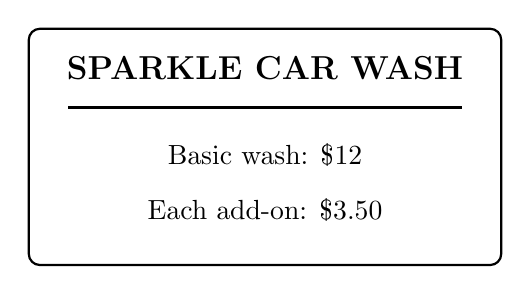
\begin{tikzpicture}
  \draw[thick, rounded corners] (0,0) rectangle (6,3);
  \node[font=\bfseries\large] at (3,2.5) {SPARKLE CAR WASH};
  \draw[thick] (0.5,2) -- (5.5,2);
  \node[align=left] at (3,1.4) {Basic wash: \$12};
  \node[align=left] at (3,0.7) {Each add-on: \$3.50};
\end{tikzpicture}
\end{center}
\end{questionText}
\choiceA{$12a + 3.50$}
\choiceB{$3.50a + 12$}
\choiceC{$15.50a$}
\choiceD{$12 + 3.50 + a$}
\correctAnswer{B}
\explanation{The basic wash is $\$12$ and each add-on costs $\$3.50$, so $a$ add-ons cost $3.50a$. Total: $3.50a + 12$.}
\end{practiceQuestion}

% --- Graphical Short Answer Questions (3) ---

\begin{practiceQuestion}{4-1-q25}{gsa}
\begin{questionText}
The table shows the total cost of renting a canoe for different numbers of hours.

\begin{center}
\begin{tabular}{|c|c|}
\hline
\textbf{Hours ($h$)} & \textbf{Cost (\$)} \\
\hline
$1$ & $\$18$ \\
\hline
$2$ & $\$26$ \\
\hline
$3$ & $\$34$ \\
\hline
$4$ & $\$42$ \\
\hline
\end{tabular}
\end{center}

Write an expression for the rental cost for $h$ hours and find the cost for $6$ hours.
\end{questionText}
\correctAnswer{$8h + 10$; $\$58$}
\explanation{Cost increases by $\$8$ per hour. When $h = 0$ the cost would be $\$10$ (the starting fee). Expression: $8h + 10$. For $h = 6$: $8(6) + 10 = 48 + 10 = \$58$.}
\end{practiceQuestion}

\begin{practiceQuestion}{4-1-q26}{gsa}
\begin{questionText}
An input-output machine applies a rule to each input value. Complete the table and write the rule.

\begin{center}
\begin{tikzpicture}[scale=0.8]
  \node[draw, rounded corners, fill=funOrange!20, minimum width=2.5cm, minimum height=1cm] at (3,0) {\textbf{Rule: ?}};
  \draw[->, thick] (0,0) -- (1.5,0);
  \draw[->, thick] (4.5,0) -- (6,0);
  \node[left] at (0,0) {\textbf{Input}};
  \node[right] at (6,0) {\textbf{Output}};
  \node at (0,-1.5) {$2$}; \node at (6,-1.5) {$-1$};
  \node at (0,-2.2) {$4$}; \node at (6,-2.2) {$5$};
  \node at (0,-2.9) {$6$}; \node at (6,-2.9) {$11$};
  \node at (0,-3.6) {$10$}; \node at (6,-3.6) {?};
\end{tikzpicture}
\end{center}
\end{questionText}
\correctAnswer{Rule: $3x - 7$; output for $10$ is $23$}
\explanation{Test $x = 2$: $3(2) - 7 = -1$ \checkmark. Test $x = 4$: $3(4) - 7 = 5$ \checkmark. The rule is $3x - 7$. For $x = 10$: $3(10) - 7 = 23$.}
\end{practiceQuestion}

\begin{practiceQuestion}{4-1-q27}{gsa}
\begin{questionText}
A recipe card shows the ingredients needed per batch of cookies. Write an expression for the total cups of flour needed for $b$ batches, and find the amount for $5$ batches.

\begin{center}
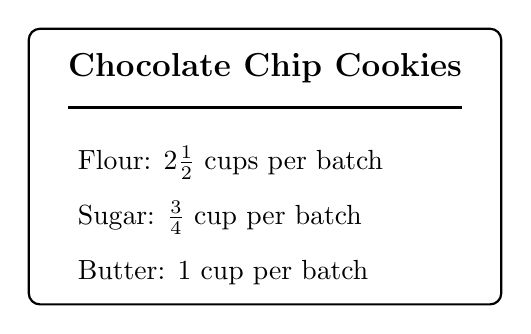
\begin{tikzpicture}
  \draw[thick, rounded corners] (0,0) rectangle (6,3.5);
  \node[font=\bfseries\large] at (3,3) {Chocolate Chip Cookies};
  \draw[thick] (0.5,2.5) -- (5.5,2.5);
  \node[align=left, anchor=west] at (0.5,1.8) {Flour: $2\frac{1}{2}$ cups per batch};
  \node[align=left, anchor=west] at (0.5,1.1) {Sugar: $\frac{3}{4}$ cup per batch};
  \node[align=left, anchor=west] at (0.5,0.4) {Butter: $1$ cup per batch};
\end{tikzpicture}
\end{center}
\end{questionText}
\correctAnswer{$2.5b$ (or $\frac{5}{2}b$); $12.5$ cups}
\explanation{Each batch needs $2\frac{1}{2} = 2.5$ cups of flour. For $b$ batches: $2.5b$. For $b = 5$: $2.5(5) = 12.5$ cups.}
\end{practiceQuestion}
